To find the related literature a literature search query was formed. The search query was separated into three parts to obtaining more successful findings, individually focusing on a single topic. These parts are Android, maintainability and methods/technologies, respectively. Fig. \ref{fig:lit_review_research_query} presents the visualization of the search query.
\begin{figure}[ht!] 
    \centering
    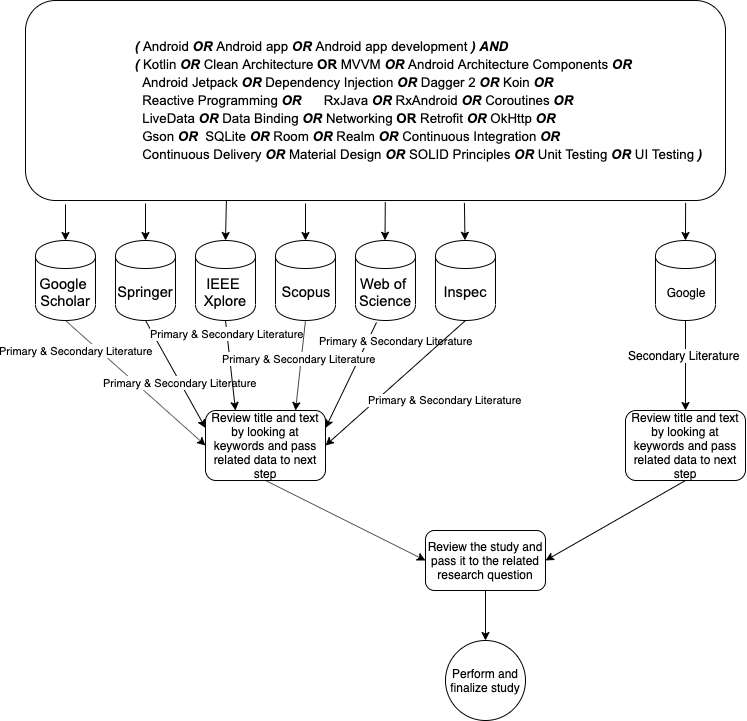
\includegraphics[scale=0.45]{figures/research_query.png}
    \caption{Literature review visualization}
    \label{fig:lit_review_research_query}
\end{figure}
\FloatBarrier

A set of criteria has been determined to increase the accuracy of the results obtained from the search query and to filter out possible irrelevant studies among the results. While determining the criteria, issues such as the language of the reviewed studies, their up-to-dateness and their relevance to native Android development were taken into consideration. The inclusion and exclusion criteria are shown in Table \ref{fig:lit_review_research_query_criteria}.
\begin{table}[htb]
    \centering
    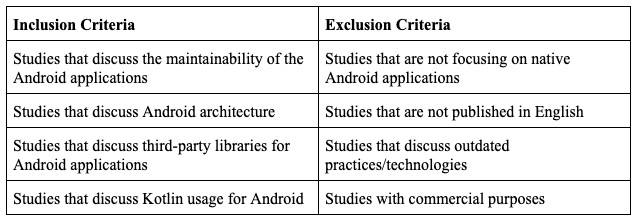
\includegraphics[scale=0.5]{figures/research_query_criteria.png}
    \caption{Inclusion and exclusion criteria}
    \label{fig:lit_review_research_query_criteria}
\end{table}